\documentclass[a4paper]{article}

\usepackage[utf8]{inputenc}
\usepackage[portuguese]{babel}
\usepackage{a4wide}
\usepackage[pdftex]{hyperref}
\usepackage{graphicx}
\usepackage{wrapfig}
\usepackage{amsmath}
\usepackage{verbatim}
\usepackage{caption}
\usepackage{subcaption}
\usepackage{float}



\begin{document}

\begin{titlepage}
\begin{center}



\includegraphics[width=0.6\textwidth]{logo.jpg}\\[0.5cm]

{\large Universidade do Minho - Escola de Engenharia}\\[0.5cm]

{\large Relatório do trabalho prático de Sistemas Distribuídos}\\[0.5cm]

% Title
\rule{\linewidth}{0.5mm} \\[0.4cm]
{ \huge \bfseries Matchmaking num jogo online \\[0.4cm] }
\rule{\linewidth}{0.5mm} \\[1.5cm]

% Author and supervisor
\noindent
\begin{minipage}{0.4\textwidth}
  \begin{flushleft} \large
    \emph{Autores :}\\
    Daniel Maia \textsc{(A77531)}\\
    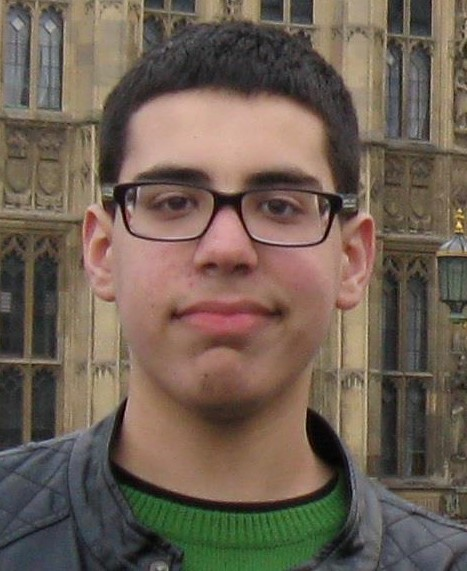
\includegraphics[width=1.5cm]{daniel.jpg}\break
    Diogo Silva\textsc{(A78034)}\\
    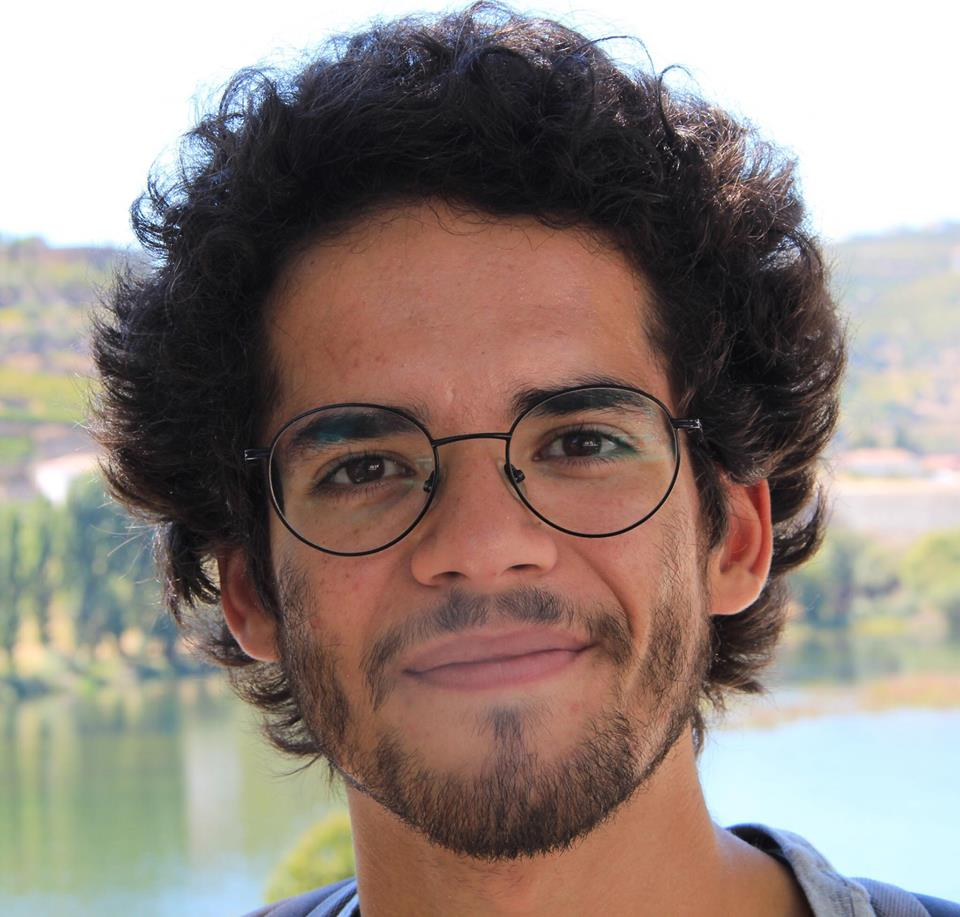
\includegraphics[width=1.5cm]{afonso.jpg}\break
    Marco Silva\textsc{(A79607)}\\
    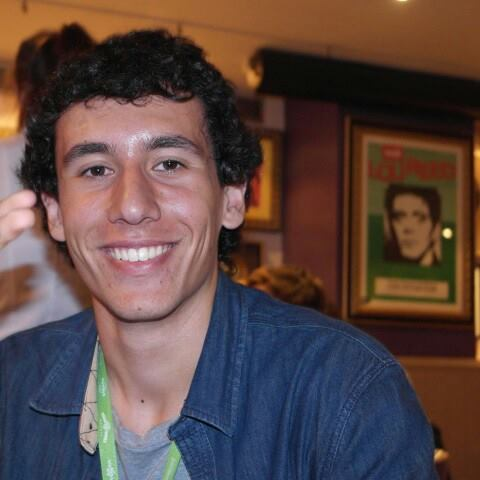
\includegraphics[width=1.5cm]{marco.jpg}\break
  \end{flushleft}
\end{minipage}%
\vfill

% Bottom of the page
{\large Versão 1.0 \\ \today}

\end{center}
\end{titlepage}




%\begin{abstract}

%\hspace{3mm} 

%\end{abstract}

%\pagebreak
\tableofcontents

\pagebreak
\section{Introdução}
\label{sec:1}

\hspace{3mm} Neste relatório será apresentado um projeto desenvolvido no âmbito da Unidade Curricular de Sistemas Distribuídos da Universidade do Minho.

\par Este projeto consiste num sistema de gestão de jogadores de um servidor \emph{online} desde o seu registo, autenticação até à disputa do jogo em si. É de salientar que neste projeto no que diz respeito ao jogo em si, é feita apenas uma geração de um resultado aleatório definindo assim a equipa vencedora e a equipa perdedora.



%------------------------------------------------------------------------

\section{Descrição do problema}
\label{sec:2}

\hspace{3mm} A proposta de trabalho dada para o projeto é o da implementação de uma aplicação distribuída para \textit{matchmaking} num jogo \textit{online}, num estilo semelhante a videojogos tais como Overwatch ou Paladins. Esta aplicação terá a capacidade de, nomeadamente, formar automaticamente duas equipas por partida e permitir a cada jogador um intervalo de tempo para escolher uma personagem, referida como herói, antes da partida iniciar.

\par Cada equipa será constituída por 5 jogadores, cada um com uma classificação pessoal. Esta classificação, determinada pelas vitórias e derrotas sofridas no jogo, terá um valor inteiro entre 0 e 9, e terá no máximo uma diferença unitária entre todos os jogadores de uma dada partida. Tendo encontrado 10 jogadores disponíveis com classificações semelhantes, o servidor dividi-los-á em equipas equilibradas de acordo com as classificações dos mesmos. Para que esta classificação seja guardada, será implementado um sistema de registo e autenticação. Com um nome de utilizador e uma palavra passe, o servidor autentica o jogador sempre que este estabelece ligação ao mesmo.

\par Tendo as duas equipas feitas, os jogadores procederão à fase da escolha dos heróis, dos quais existem 30. Cada jogador poderá escolher qualquer um, desde que este não tenha ainda sido selecionado por outro jogador da mesma equipa. Como tal, cada jogador poderá ver as escolhas de heróis dos elementos da mesma equipa. Qualquer jogador poderá selecionar um herói diferente, caso mude de ideias. Após 30 segundos, a fase de escolha será dada como terminada. Se algum jogador da partida não tiver escolhido um herói, a partida é abortada e cada jogador terá de selecionar a opção de jogar uma vez mais. Caso contrário, será mostrada a composição de ambas equipas a todos os jogadores da partida, nomeadamente o nome de utilizador de cada jogador e respetivo herói. É depois simulada uma partida, cujo resultado aleatório será utilizado para atualizar a classificação de cada jogador, subindo com cada vitória e descendo com cada derrota.

\par Para aceder ao servidor, cada jogador terá acesso a um programa Cliente, com o qual acederá a um Servidor \textit{multithreaded} através de \textit{sockets} TCP. Em concordância com a proposta do trabalho, o protocolo entre os dois será baseado em texto, orientado à linha, e cada \textit{thread} do Servidor escreverá em um e só um \textit{socket}.


\pagebreak
\clearpage
%--------------------------------------------------------------------------

\section{Conceção da Solução}
\label{sec:3}

\subsection{Registo e login}
\label{sec:3.1}

\hspace{3mm} Ao ser estabelecida a ligação ao Servidor, o Cliente será apresentado com as opções de fazer o registo no jogo, autenticar a sua identidade, supondo que já tenha feito o registo, e sair do jogo, terminando a ligação e encerrando o programa Cliente. Para guardar os registos dos jogadores, será necessário guardá-los no Servidor, num \textit{HashMap} cuja chave será o nome de utilizador e cujo valor será um objeto Jogador no qual estará guardada a informação do mesmo.

\par Ao fazer o registo, o Cliente terá de introduzir um nome de utilizador que será único ao mesmo. Caso o nome de utilizador escolhido já existir em registo, o Servidor informará o Cliente da ocorrência e pedirá um nome de utilizador alternativo. Sendo introduzido um nome de utilizador válido, será de seguida introduzida uma palavra passe pelo Cliente, de modo a que este possa assegurar que apenas o jogador em questão possa aceder ao seu perfil, o qual pode ser acedido de qualquer programa Cliente. Após o registo, o jogador é de imediato autenticado, de modo a dar conveniência ao mesmo.

\par Para fazer a autenticação de um jogador, é necessário que este tenha já feito registo no jogo. Para ser autenticado, um jogador necessita apenas introduzir o seu nome de utilizador e palavra passe. Caso alguma destas estiver errada, o Servidor informará o Cliente deste erro e dará outra oportunidade de autenticar o jogador. 



\subsection{Matchmaking}
\label{sec:3.2}

\hspace{3mm} O \textit{Matchmaking} consiste na seleção dos jogadores que indicaram que pretendiam jogar seguindo algumas das regras que foram impostas na descrição do projeto como por exemplo a impossibilidade de numa sala de jogo existirem diferenças superiores a 1 unidade no que toca aos níveis dos jogadores intervenientes.

\par Este sistema de \textit{matchmaking} para que a seleção dos jogadores seja feita da forma mais eficiente possível define zonas de agrupação de jogadores para cada um dos níveis possíveis exceto o nível 9. Assim, cada um dos jogadores pode entrar numa sala com o índice do seu nível ou na sala com índice imediatamente abaixo do seu nível. Nos casos de jogadores com nível 0 e 9, estes entram sempre em sala com índice 0 e 8 respetivamente. Finalmente, a decisão entre as duas salas possíveis é feita com base na ocupação de cada uma das salas, dando sempre a prioridade à sala que se encontra mais perto de estar completa, ou seja, com mais jogadores.

\par Quando o número de jogadores necessários para passar à proxima fase é atingido (10), todos os jogadores passam à fase seguinte (construção das equipas).


\subsection{Fazer equipas}
\label{sec:3.3}

\hspace{3mm} Para que o jogo seja o mais justo possível, foi desenvolvido um algoritmo para a construção das equipas que tem por base os níveis dos jogadores construido assim duas equipas com o nível médio dos níveis dos jogadores o mais próximo possível.

\par O algoritmo verifica numa primeira fase se o número de jogadores em cada uma das equipas é o mesmo e se se verificar, caso o nível do jogador seja o maior da sala, então o jogador é inserido na equipa que tem um menor número de jogadores com o nível máximo da sala. Ainda com o mesmo número de jogadores em cada uma das equipas mas o jogador tem o menor nível possível na sala, então este é inserido na equipa que tem mais jogadores com o nível máximo na sala. Finalmente, no caso em que o número de jogadores em cada uma das equipas é desigual, então o jogador é inserido na equipa com o menor número de jogadores independentemente do seu nível.

\subsection{Escolha de heróis}
\label{sec:3.4}
\hspace{3mm} A fase de escolha dos heróis permite aos jogadores escolherem os heróis com os quais pretendem jogar. No entanto, essa escolha deve ser transmitida para todos os jogadores da sua equipa para que estes tomem conhecimento da decisão. Os jogadores que pertencem à mesma partida mas à equipa contrária não devem ter acesso à conversação realizada pela equipa contrária.

Desta forma, a solução que permite implementar esta funcionalidade é constituída por um \texttt{ChatEscolhaHerois}, um \texttt{Timer}, um \texttt{TrataJogadorEscrita}, um \texttt{TrataJogadorLeitura} e um \texttt{ClientWorker}. Na realidade a classe \texttt{ChatEscolhaHerois} encontra-se armazenada pelo número da sala e número de partida numa estrutura definida pela classe \texttt{HashChats}. Esta classe classe organiza cada chat de acordo com o número da sala e partida, visto que estes dois valores identificam únicamente uma partida. Para tal utiliza a seguinte estrutura: \texttt{Map<Integer, Map<Integer, ChatEscolhaHerois>>}. Na prática todas as threads confirmam que já têm um chat pronto para o seu jogo. A primeira thread a perceber que ainda não existe, ficam incumbida de criar uma instância da classe \texttt{ChatEscolhaHerois} e coloca-la na \textit{hash}. As restantes threads apenas acedem ao chat criado.

%ChatEscolhaHerois
A classe \texttt{ChatEscolhaHerois} é responsável por armazenar toda a informação relacionada com o chat, assim como com a escolha dos heróis. Deste modo, são utilizadas dois \textit{HashMaps}, um para cada equipa visto que os heróis entre equipas podem repetir, com uma chave identificada pelo nome do herói escolhido e o valor com o username do jogador que o escolheu. Cada \textit{HashMap} tem um \textit{lock} pois é uma estrutura partilhada por várias \textit{threads}, que sofre múltiplas inserções e remoções concorrentemente. O método de exclusão mútua utilizado para proteger os \textit{HashMaps} anteriores foi conseguido com a ajuda dos \textit{ReentrantLocks}, um por cada \textit{Map}. Efetivamente, esta decisão adveio do facto do método \texttt{escolheHeroi} ser utilizado pelas duas equipas indiferenciadamente. Caso este método fosse colocado como \texttt{synchronized} as duas equipas tornavam-se dependentes uma da outra na escolha dos heróis. Com os \textit{locks} consegue-se isolar a escolha das duas equipas, ou seja, enquanto uma equipa escolhe um herói a outra pode estar a fazê-lo visto que escrevem em estruturas diferentes, apenas utilizam o mesmo método, sendo que dentro da mesma equipa a concorrência é controlada e apenas um jogador de cada vez consuma a sua escolha. 
%Esta parte ainda tenho que ver porque deviamos ter um chat para cada equipa!!!
Além disso, a classe conta com a variável \texttt{log} do tipo \texttt{ArrayList<String>}, que é responsável por armazenar a conversa...

%TrataJogadorEscrita/Leitura & Estrutura utilizada
As classes \texttt{TrataJogadorEscrita} e \texttt{TrataJogadorLeitura} são o resultado do método utilizado para implementar comunicação entre o jogador e o servidor de forma a obter um chat funcional. Efetivamente, o \texttt{TrataJogadorEscrita} é responsável por ler da variável \texttt{log} mencionada acima, ou seja, do chat e transmiti-la para o jogador que lhe corresponde. Na verdade, a thread que anima esta classe encontra-se adormecida enquanto não existe alteração no chat. Mal um nova entrada seja introduzida, a thread acorda e reencaminha as novas entradas. Dado que cada jogador tem o seu \texttt{TrataJogadorEscrita} então é feito o \textit{broadcast} da informação do chat para todos os jogadores. A classe \texttt{TrataJogadorLeitura} é responsável maioritariamente por ler o herói escolhido pelo jogador e enviá-lo para o \texttt{log}. Além disso, realiza algum processamento nos dados que recebe do jogador, nomeadamente se este escolheu um herói que se encontra indisponível no momento é de imediato dito ao cliente que tem de refazer a sua escolha.

A classe \texttt{Timer} tem uma instância para cada partida. O objetivo desta é não deixar que a escolha dos heróis ultrapasse os trinta segundos. Cada instância é guardada numa hash que tem como chaves a sala e a partida. À semelhança do que acontece com o chat, a primeira thread a perceber que ainda não foi criado um \texttt{Timer} para a sua partida procede à sua criação. No final dos trinta segundos é colocado uma mensagem no chat para que esta ao ser difundida vá terminando todas as threads envolvidas no chat.

Além disso, no lado do jogador além da classe \texttt{Cliente} é cridada um \texttt{ClientWorker}. Este fica apenas responsável por ler o que vem do servidor e imprime no ecrã do jogador.

Reunindo todos os recursos é possível perceber pela figura \ref{} a conjugação de todos os componentes que o chat envolve. 

Inicialmente, é criada a estrutura do chat. De seguida são criadas as threads \texttt{TrataJogadorEscrita}, \texttt{TrataJogadorLeitura} e do \texttt{Timer}. Do lado do cliente é criado o \texttt{ClientWorker}. Neste momento o jogador encontra-se na posição de escolher o herói com o qual pretende jogar e envia a sua escolha ao \texttt{TrataJogadorLeitura}. Após processar o pedido do jogador, se estiver tudo correto, este é enviado ao \texttt{ChatEscolhaHerois} para que este efetiva a escolha do jogador. De seguida, acorda todas as threads do \texttt{TrataJogadorEscrita} e estas enviam a escolha do jogador a todos os outros jogadores da mesma equipa. Quando essa informação chega ao \texttt{ClientWorker} este simplesmente imprime a escolha no ecrã do jogador.

No final dos trinta segundos, a thread responsável por animar o \texttt{Timer} envio o código \textbf{timeout} ao chat para que este saiba que o tempo de escolha dos heróis acabou. Consequentemente, a thread \texttt{TrataJogadorEscrita} acorda com a nova entrada e confirma que todos os jogadores escolheram um herói. Caso alguém não tenha escolhido, então a variável \texttt{jogar} é colocada a \texttt{false} e o código \textbf{timeout} é enviado para o \texttt{ClientWorker}. Caso contrário, a variável \texttt{start} é colocada a \texttt{true} e o código \textbf{start} é enviado ao \texttt{ClientWorker}. No final a thread do \texttt{TrataJogadorEscrita} termina. O \texttt{ClientWorker} recebe o código e consoante o seu valor coloca ou não a variável jogar do lado do jogador a \texttt{true}. De seguida, envia o código \textbf{morre} ao \texttt{TrataJogadorLeitura} para este terminar e ambos terminam a sua execução.

%Figura do esquema geral

\subsection{Cálculo dos resultados}
\label{sec:3.5}
\hspace{3mm} O cálculo de resultados é realizado de forma aleatória dado que não se encontra implementado o jogo propriamente.

De facto, a classe que armazena todas as instâncias de \texttt{Jogo} é a \texttt{HashJogos}. Mais uma vez, à semelhança do que acontece com o chat utiliza-se um \textit{HashMap} com as chaves sendo a sala e a partida, para armazenar todos os jogos que são realizados. A primeira thread cria a instância de jogo. A última coloca o jogo a correr, ou seja, é a que dispulta o cálculo do resultado. Para o efeito é usado a expressão \texttt{this.resultado = (Math.random()<0.5)?1:2;}, que permite obter um resultado aleatório entre 1 e 2. Sendo que 1 significa que a equipa 1 ganhou e 2 significa que a equipa 2 ganhou. 

Por fim, o resultado é guardado na instância de Jogo para mais tarde ser consultado e consequentemente enviado para o jogador.

%--------------------------------------------------------------------------

\section{Conclusões}
\label{sec:4}

\hspace{3mm} Este projecto encontra-se finalizado. Contudo, alguns ajustes podem ser feitos e certas funcionalidades podem ser certamente melhoradas.
Nomeadamente, no que toca ao número de threads usadas para realizar o matchmaking, este encontra-se fixo em 9 threads, uma por cada rank. No entanto, com um número elevado de jogadores esta abordagem pode reduzir a performance do jogo e os tempos de espera dos jogadores pode aumentar consideravelmente. Uma possível proposta seria tornar o número de threads, responsáveis por esta funcionalidade, dinâmico. Quanto maior o número de jogadores em espera para jogar, maior seria o número de threads ativas e vice-versa. Desta forma, o matchmaking conseguiria obter tempos de espera menores.

Além disso, outro ponto que deveria ser abordado numa próxima etapa seria melhorar a interface com o utilizador. De facto, na escolha dos heróis, devido à concorrência existente entre os vários jogadores, o chat que estes utilizam para o efeito encontra-se desordenado e nada intuitivo. Sendo este um dos principais aspetos a melhorar.

Concluindo, o projeto decorreu sem grandes sobressaltos e os tempos de resposta mesmo com 500 jogadores foram satisfatórios. De recordar que estes resultados não seriam possiveis se não fosse utilizada uma abordagem concorrente ao problema, ou seja, utilizando o modelo cliente/servidor com a ajuda de sockets, threads e controlo de concorrência.

\end{document}
